% Day 1 notes, SC Quantathon v3 Bootcamp. Build: latexmk -pdf notes.tex
\documentclass[11pt]{article}

\usepackage[margin=1in]{geometry}
\usepackage{lmodern}
\usepackage[T1]{fontenc}
\usepackage{microtype}
\usepackage{amsmath,amssymb}
\usepackage{braket}
\usepackage{graphicx}
\usepackage{booktabs}
\usepackage{caption}
\usepackage{listings}
\usepackage{xcolor}
\usepackage[hidelinks]{hyperref}

\captionsetup{font=small,labelfont=bf}
\graphicspath{{figures/}}

\lstset{
  language=Python,
  basicstyle=\ttfamily\small,
  keywordstyle=\color{blue!60!black},
  commentstyle=\color{gray},
  stringstyle=\color{green!40!black},
  showstringspaces=false,
  frame=single,
  framerule=0.3pt,
  rulecolor=\color{gray!50},
  xleftmargin=1em,
  aboveskip=0.6em,
  belowskip=0.6em,
}

\newcommand{\code}[1]{\texttt{#1}}


\title{Day 1: Setup, Python Refresher, and Your First Circuit}
\author{SC Quantathon v3 Bootcamp \\ Clemson Quantum Club}
\date{}

\begin{document}
\maketitle

\noindent
These notes follow the Day~1 notebook section by section. The notebook is where you run things; these pages give the explanations, the equations, and the figures behind each step, so that either one can be read on its own.


\section{Setup}

The notebook runs in two places. Locally, the repository's \code{requirements.txt} pins Qiskit~2.5, the Aer simulator, and the IBM runtime client into a conda environment. On qBraid Lab those packages are preinstalled. Every cell behaves the same on both.

Two accounts matter this week. The IBM Quantum Open Plan gives ten minutes of QPU time per 28-day rolling window on real superconducting processors, and the notebook's section~2 stores its API key on disk once under the name \code{scqv3} so that no later notebook needs the key in a cell. The qBraid account is where the hackathon credits live; Day~3 covers that platform.

\section{Python essentials}

Everything in the bootcamp is built from a small set of Python pieces. Table~\ref{tab:python} lists the ones that appear in every later notebook, with the reason each one matters here.

\begin{table}[h]
\centering
\small
\begin{tabular}{@{}lll@{}}
\toprule
Construct & Example & Where it shows up \\
\midrule
list & \code{["00", "01", "10", "11"]} & the possible outcomes of a circuit \\
dictionary & \code{\{"00": 503, "11": 497\}} & every measurement result Qiskit returns \\
\code{.get(key, 0)} & \code{counts.get("01", 0)} & reading an outcome that may not have occurred \\
function & \code{def probability\_of\_zero(...)} & the exercises from Day~2 on \\
f-string & \code{f"\{p:.3f\}"} & printing probabilities to three decimals \\
numpy array & \code{np.array([1, 0])} & qubit states and gate matrices \\
\code{@} & \code{U @ psi} & applying a gate to a state \\
\code{.conj().T} & \code{U.conj().T} & the conjugate transpose $U^\dagger$ \\
\code{np.allclose} & \code{np.allclose(A, B)} & comparing floating-point arrays \\
\bottomrule
\end{tabular}
\caption{The Python and numpy constructs the bootcamp uses.}
\label{tab:python}
\end{table}

\subsection{Complex numbers}

A complex number is $z = x + iy$ with $i^2 = -1$; Python writes $i$ as \code{1j}. Three quantities are used constantly from Day~2 onward. The magnitude, the conjugate, and their product:
\begin{equation}
|z| = \sqrt{x^2 + y^2}, \qquad \bar z = x - iy, \qquad z\bar z = x^2 + y^2 = |z|^2 .
\end{equation}
Any complex number of magnitude one can be written as a point on the unit circle,
\begin{equation}
e^{i\phi} = \cos\phi + i\sin\phi, \qquad |e^{i\phi}| = 1 \ \text{for every real } \phi,
\end{equation}
which is what \code{np.exp(1j * phi)} computes. In numpy, \code{abs(z)}, \code{np.conj(z)}, and \code{np.angle(z)} return $|z|$, $\bar z$, and $\phi$.

\subsection{Vectors and matrices}

A vector $v$ with complex entries is \emph{normalized} when
\begin{equation}
\sum_i |v_i|^2 = 1 .
\label{eq:norm}
\end{equation}
Dividing any nonzero vector by $\sqrt{\sum_i |v_i|^2}$ produces a normalized one. Matrices act on vectors by the product \code{M @ v}, and the conjugate transpose $M^\dagger$ is \code{M.conj().T}. The notebook's example is a quarter turn of the plane,
\begin{equation}
R = \begin{pmatrix} 0 & -1 \\ 1 & 0 \end{pmatrix}, \qquad
R \begin{pmatrix} 1 \\ 0 \end{pmatrix} = \begin{pmatrix} 0 \\ 1 \end{pmatrix}, \qquad
R^{\mathsf T} R = I ,
\end{equation}
so undoing the rotation is the same as applying the transpose. Quantum gates on Day~2 will be exactly this kind of matrix, with $R^\dagger R = I$ in place of $R^{\mathsf T} R = I$.

One habit matters from the first cell on: never test floating-point results with \code{==}. In binary floating point $0.1 + 0.2$ is not $0.3$ but $0.30000000000000004$, and a normalized vector computed by dividing by a square root has a norm of $1$ only to about 16 digits. \code{np.allclose(a, b)} compares two arrays to within a tolerance (by default $10^{-8}$ absolute plus $10^{-5}$ relative) and is what every Checkpoint in the bootcamp uses; \code{np.isclose} does the same for single numbers.

\section{Bits and gates}

A bit is always exactly one of two values, 0 or 1. Reading it does not change it. A classical gate is a lookup table from input bits to output bits; Table~\ref{tab:gates} shows the two simplest ones.

\begin{table}[h]
\centering
\small
\begin{tabular}{@{}cc@{}}
\toprule
$a$ & $\mathrm{NOT}\,a$ \\
\midrule
0 & 1 \\
1 & 0 \\
\bottomrule
\end{tabular}
\qquad\qquad
\begin{tabular}{@{}ccc@{}}
\toprule
$a$ & $b$ & $a \wedge b$ \\
\midrule
0 & 0 & 0 \\
0 & 1 & 0 \\
1 & 0 & 0 \\
1 & 1 & 1 \\
\bottomrule
\end{tabular}
\qquad\qquad
\begin{tabular}{@{}ccc@{}}
\toprule
$a$ & $b$ & $a \oplus b$ \\
\midrule
0 & 0 & 0 \\
0 & 1 & 1 \\
1 & 0 & 1 \\
1 & 1 & 0 \\
\bottomrule
\end{tabular}
\caption{NOT, AND, and XOR as lookup tables.}
\label{tab:gates}
\end{table}

NOT is \emph{reversible}: applying it twice returns the input. AND is not. Given the output 0, three different input pairs could have produced it, so the inputs are lost. Most classical gates discard information this way.

XOR alone is also irreversible, since $(0,1)$ and $(1,0)$ both give 1. But the two-output map
\begin{equation}
(a, b) \;\longmapsto\; (a,\; a \oplus b)
\label{eq:cnot}
\end{equation}
sends the four inputs to four distinct outputs, so it can be undone. In words: keep the first bit, and flip the second bit when the first is 1. Every quantum gate is reversible, and Eq.~\eqref{eq:cnot} is the truth table of the two-qubit gate called CNOT that appears on Day~4.

There is a counting argument behind this. A gate on $n$ bits has $2^n$ possible inputs. It is reversible when it sends them to $2^n$ distinct outputs; with as many output bits as input bits, that means its table is a \emph{permutation} of the $2^n$ bitstrings. NOT permutes two strings, Eq.~\eqref{eq:cnot} permutes four (writing the pair as $ab$, it swaps $10$ and $11$ and fixes the rest), and AND sends four inputs onto two outputs and so cannot be a permutation. The quantum rule of Day~2, that a gate is a unitary matrix, is the same requirement stated for amplitudes instead of bits: a unitary sends distinct states to distinct states and has an inverse.

\section{Qubits, in words}

Until it is measured, a qubit is a weighted blend of 0 and 1 called a \emph{superposition}. Measuring it forces one of the two answers and destroys the blend. Because a single measurement returns a single bit, a quantum program is read by running it many times and looking at the histogram of outcomes.

A qubit also carries a \emph{phase}, a sign (more generally an angle) attached to each of the two possibilities. Signs can cancel, and that cancellation, called \emph{interference}, is what a classical coin cannot do. Day~2 writes the phase down as a complex number.

Three ingredients separate a quantum computer from a classical one:
\begin{itemize}
\item \textbf{Superposition.} One qubit holds a blend of 0 and 1; $n$ qubits hold a blend of all $2^n$ bitstrings.
\item \textbf{Entanglement.} Qubits whose outcomes are linked, so that measuring one tells you the other.
\item \textbf{Interference.} Phases arranged so that wrong answers cancel and the right one adds up.
\end{itemize}
A quantum algorithm uses all three and then measures. Today's circuit uses only the first.

\section{The quantum random number generator}
\label{sec:qrng}

\subsection{The circuit}

The smallest useful quantum program has one qubit, one gate, and one measurement (Figure~\ref{fig:circuit}). The qubit starts in the state written $\ket{0}$. The Hadamard gate $H$ turns it into an equal superposition of $\ket{0}$ and $\ket{1}$, and the measurement returns 0 or 1:
\begin{equation}
\ket{0} \;\xrightarrow{\;H\;}\; \frac{1}{\sqrt 2}\big(\ket{0} + \ket{1}\big) \;\xrightarrow{\ \text{measure}\ }\; 0 \text{ or } 1, \quad \text{each with probability } \tfrac12 .
\label{eq:qrng}
\end{equation}
The factor $1/\sqrt2$ is there so the state is normalized in the sense of Eq.~\eqref{eq:norm}: the probabilities are the squared magnitudes of the coefficients, $|1/\sqrt2|^2 = 1/2$ each. Day~2 makes this precise.

\begin{figure}[h]
\centering
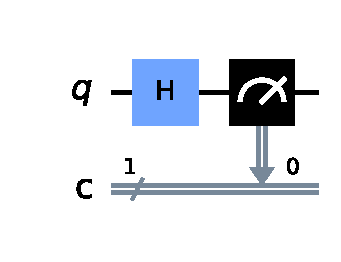
\includegraphics[width=0.32\textwidth]{qrng_circuit}
\caption{The one-qubit random number generator as the notebook draws it. Read left to right: the qubit $q$ starts in $\ket{0}$, passes through $H$, and is measured into the classical bit $c$.}
\label{fig:circuit}
\end{figure}

In Qiskit the circuit is an object that operations are appended to, one per line:
\begin{lstlisting}
qc = QuantumCircuit(1, 1)     # 1 qubit, 1 classical bit
qc.h(0)                       # Hadamard on qubit 0
qc.measure(0, 0)              # measure qubit 0 into classical bit 0
\end{lstlisting}

\subsection{Running it}

A simulator is a classical program that computes what the circuit would output. Running the circuit for a number of \emph{shots} returns a dictionary from outcome to count:
\begin{lstlisting}
result = AerSimulator().run(qc, shots=1000).result()
counts = result.get_counts()        # e.g. {'0': 489, '1': 511}
\end{lstlisting}
Those two lines, together with the three above, are the pattern for every circuit in the bootcamp: build, run, read the counts. The notebook's run with 1000 shots gave 503 zeros and 497 ones (Figure~\ref{fig:simhist}); the simulator there is unseeded, so your own run will differ by a few counts.

\begin{figure}[h]
\centering
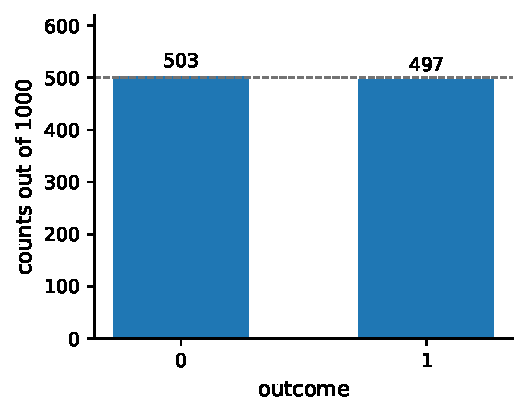
\includegraphics[width=0.42\textwidth]{qrng_simulator}
\caption{The circuit of Figure~\ref{fig:circuit} on the Aer simulator, 1000 shots. The dashed line is the ideal 500.}
\label{fig:simhist}
\end{figure}

\subsection{Shots and statistics}

Each shot is an independent draw that gives 0 with probability $p$. Over $N$ shots the number of zeros $k$ follows a binomial distribution with mean and variance
\begin{equation}
\mathbb{E}[k] = Np, \qquad \operatorname{Var}[k] = Np(1-p),
\end{equation}
so the count fluctuates by one standard deviation
\begin{equation}
\sigma = \sqrt{Np(1-p)} .
\label{eq:sigma}
\end{equation}
For the fair coin of Eq.~\eqref{eq:qrng}, $p = 1/2$, and with $N = 1000$ this is $\sigma = \sqrt{250} \approx 16$ counts. A result of 484 or 516 zeros is ordinary. A result of 400 is more than six standard deviations away and would mean the circuit is not what you think it is.

The natural estimate of the probability is $\hat p = k/N$, whose standard deviation is
\begin{equation}
\sigma_{\hat p} = \frac{\sigma}{N} = \sqrt{\frac{p(1-p)}{N}} .
\label{eq:sigma_p}
\end{equation}
Precision improves as $1/\sqrt N$: ten times more shots buys about three times more precision. Turned around, Eq.~\eqref{eq:sigma_p} says how many shots a target precision costs: $N = p(1-p)/\sigma_{\hat p}^2$, which for a fair coin is 2500 shots for $\sigma_{\hat p} = 0.01$ and 250\,000 shots for $0.001$. Every extra decimal place costs a hundred times more shots, and on a real processor shots are the currency, ten minutes of them per month on the Open Plan. For $N$ of a few dozen or more the binomial distribution is close to a Gaussian, so the usual rule applies: about 68\% of runs land within one $\sigma$ of the mean, 95\% within two, and 99.7\% within three, and a six-$\sigma$ result like 400 zeros has a probability below $10^{-8}$. The notebook's section 7.3 gave $\hat p = 0.700,\ 0.460,\ 0.497,\ 0.502$ at $N = 10,\ 100,\ 1000,\ 10000$: the estimate wanders at small $N$ (seven zeros in ten is a 1.3-$\sigma$ event, nothing unusual) and settles toward $1/2$ as Eq.~\eqref{eq:sigma_p} says it should. Figure~\ref{fig:convergence} shows those four runs against a seeded sweep over four decades of $N$.

\begin{figure}[h]
\centering
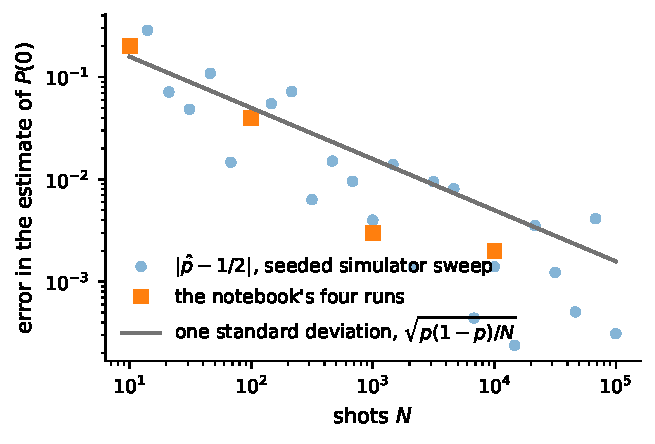
\includegraphics[width=0.6\textwidth]{shots_convergence}
\caption{The error in the estimated $P(0)$ against the number of shots: the notebook's four runs (squares) and a seeded sweep (circles). The line is Eq.~\eqref{eq:sigma_p} with $p = 1/2$. Individual points scatter above and below it, as one standard deviation should.}
\label{fig:convergence}
\end{figure}

\subsection{Where the randomness comes from}

Python's \code{random} module is a pseudorandom generator: seed it with the same number twice and it repeats the same sequence forever. The Aer simulator is also a classical program, so it accepts a seed too, and \code{AerSimulator(seed\_simulator=1)} reproduces its outcomes exactly. The notebook demonstrates both.

Only on real hardware is the outcome undetermined before the measurement takes place. The simulator reproduces the \emph{statistics} of Eq.~\eqref{eq:qrng} but not the physics.

The keyword \code{memory=True} asks the simulator to keep every individual shot in order, as a list of outcome strings, rather than only the totals. Joining 32 such outcomes gives a 32-character bitstring, and \code{int(bits, 2)} converts it to an integer between 0 and $2^{32} - 1$; the notebook's run produced \code{01100111111111010011000000011101}, which is 1\,744\,646\,173. Because each bit is an independent fair coin, every one of the $2^{32}$ integers is equally likely, with mean $2^{31} \approx 2.1\times10^9$; the string has no structure that distinguishes it from \code{random.getrandbits(32)}, and no statistical test can tell the two sources apart. What differs is only the origin: one is a formula seeded by a number, the other, on hardware, is a measurement whose outcome did not exist before it was made. Removing the $H$ gate, the notebook's last exercise, turns the circuit into one that always reads 0, which shows that the randomness comes from the superposition and not from the measurement itself.

\section{The same circuit on real hardware}

A real quantum processor is a chip with a fixed set of native gates. Two steps are added to the code. The \emph{transpiler} rewrites the circuit into those native gates; on IBM's superconducting chips the Hadamard is not native and becomes $R_z(\pi/2)\,\sqrt X\,R_z(\pi/2)$, three native gates that equal $H$ up to a global phase (\code{Operator.equiv} confirms it), which Day~5 explains. The $\sqrt X$ is one calibrated microwave pulse; the $R_z$ rotations are bookkeeping in the control electronics and cost no time at all. Then a \emph{Sampler} submits the rewritten circuit to the machine's queue:
\begin{lstlisting}
pm = generate_preset_pass_manager(optimization_level=1, backend=backend)
qc_isa = pm.run(qc)
job = Sampler(mode=backend).run([qc_isa], shots=1000)
counts = job.result()[0].data.c.get_counts()
\end{lstlisting}

Three ways of producing one random bit appear in the notebook: a classical coin from a seeded pseudorandom generator (section 6.2), the circuit on a simulator (section 7.2), and the same circuit on a quantum processor (this section). The processor run is the live 1000-shot job on \code{ibm\_kingston} recorded in the solutions notebook. Table~\ref{tab:three} lists the three with the distance of the count of zeros from 500 in units of the $\sigma \approx 16$ of Eq.~\eqref{eq:sigma}; Figure~\ref{fig:hardware} draws them side by side.

\begin{table}[h]
\centering
\small
\begin{tabular}{@{}llll@{}}
\toprule
source & count of 0 & count of 1 & $|{\rm count\ of\ 0} - 500| / \sigma$ \\
\midrule
classical coin, \code{rng.integers} & 484 & 516 & 1.0 \\
simulator, \code{AerSimulator} & 503 & 497 & 0.2 \\
quantum processor, \code{ibm\_kingston} & 295 & 705 & 13.0 \\
\bottomrule
\end{tabular}
\caption{One random bit, 1000 draws each, three ways.}
\label{tab:three}
\end{table}

\begin{figure}[h]
\centering
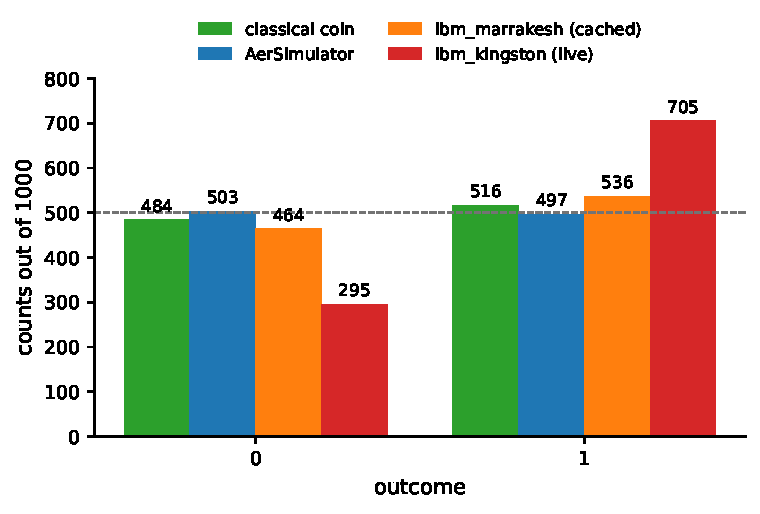
\includegraphics[width=0.62\textwidth]{classical_sim_hardware}
\caption{The three rows of Table~\ref{tab:three}. The dashed line is the ideal 500.}
\label{fig:hardware}
\end{figure}

The coin and the simulator sit within one standard deviation of 500/500, because both are exact samples from a fair distribution. They differ from each other only in what they are simulating: the coin is \code{rng.integers}, the simulator is the linear algebra of Section~\ref{sec:qrng}. Neither is physically random; both repeat given the same seed.

The hardware row is the one to look at twice. A run a couple of standard deviations from 500 would be ordinary: for a Gaussian the two-sided probability of a 2-$\sigma$ deviation is 0.046, so a fair coin does that about once in twenty runs, and one such run is no evidence of bias. The \code{ibm\_kingston} run is another matter: 295 zeros is thirteen standard deviations from 500, and no amount of shot noise produces that. The circuit ran on physical qubit~0 of the chip (the transpiler at optimization level 1 takes the first qubit rather than searching for a good one), and that qubit's calibration at the time was unremarkable: a readout error of 1.9\% in each direction, a $\sqrt X$ error of $2\times10^{-4}$, a $T_1$ of 370~$\mu$s. None of those predicts a 70/30 split. The device simply disagreed with its own calibration during that job, which happens: calibrations are snapshots taken every few hours, and a qubit can drift, or couple to a defect in its surroundings, in between. Real processors always add \emph{readout error}, the chip recording a 0 as a 1 or the reverse at the percent level, and for a 50/50 state only the asymmetry of that error shifts the counts; but a shift of twenty points is something else, and the right response is to rerun on a different qubit or machine before believing either result. Day~5 reads the calibration table, chooses qubits with it, and measures readout error directly.

\section{Summary}

\begin{itemize}
\item A bit is one of two values; a classical gate is a lookup table, and most of them are irreversible. XOR with its first input kept, Eq.~\eqref{eq:cnot}, is reversible and is the CNOT gate in disguise.
\item A qubit is a superposition of 0 and 1 until measured, and carries a phase that lets possibilities cancel. A quantum program is read as a histogram over many shots.
\item The random number generator, Eq.~\eqref{eq:qrng}, is a Hadamard followed by a measurement. In Qiskit: build the circuit, run it on a backend with some number of shots, read the counts dictionary.
\item Counts fluctuate by $\sigma = \sqrt{Np(1-p)}$ and the estimate of a probability improves as $1/\sqrt N$, Eqs.~\eqref{eq:sigma} and \eqref{eq:sigma_p}.
\item Simulators are seeded classical programs. Only measurement on real hardware is undetermined in advance.
\item Hardware adds a transpile step and a Sampler. Its counts carry readout error at the percent level, and occasionally a device error far larger than any statistics, so a single run is checked against $\sigma$ before it is believed.
\end{itemize}

\begin{thebibliography}{9}
\bibitem{helloworld} IBM Quantum, \emph{Hello World}, tutorial. \url{https://quantum.cloud.ibm.com/docs/en/tutorials/hello-world}
\bibitem{watrous} J.~Watrous, \emph{Basics of Quantum Information}, IBM Quantum Learning. \url{https://quantum.cloud.ibm.com/learning/en/courses/basics-of-quantum-information}
\bibitem{nielsen} M.~A. Nielsen and I.~L. Chuang, \emph{Quantum Computation and Quantum Information}, 10th anniversary ed. (Cambridge University Press, 2010), chapter~1.
\bibitem{qiskitdocs} Qiskit documentation. \url{https://quantum.cloud.ibm.com/docs}
\bibitem{python} The Python Tutorial. \url{https://docs.python.org/3/tutorial/}
\bibitem{numpy} NumPy quickstart. \url{https://numpy.org/doc/stable/user/quickstart.html}
\end{thebibliography}

\end{document}
